\documentclass[
11pt, % The default document font size, options: 10pt, 11pt, 12pt
%codirector, % Uncomment to add a codirector to the title page
]{charter} 




% El títulos de la memoria, se usa en la carátula y se puede usar el cualquier lugar del documento con el comando \ttitle
\titulo{Clasificación de reclamos de usuarios} 

% Nombre del posgrado, se usa en la carátula y se puede usar el cualquier lugar del documento con el comando \degreename
%\posgrado{Carrera de Especialización en Sistemas Embebidos} 
%\posgrado{Carrera de Especialización en Internet de las Cosas} 
\posgrado{Carrera de Especialización en Inteligencia Artificial}
%\posgrado{Maestría en Sistemas Embebidos} 
%\posgrado{Maestría en Internet de las cosas}

% Tu nombre, se puede usar el cualquier lugar del documento con el comando \authorname
\autor{Ing. Lucas Rivela} 

% El nombre del director y co-director, se puede usar el cualquier lugar del documento con el comando \supname y \cosupname y \pertesupname y \pertecosupname
\director{Mg. Lic. Rodrigo Cárdenas}
\pertenenciaDirector{FIUBA} 
% FIXME:NO IMPLEMENTADO EL CODIRECTOR ni su pertenencia
\codirector{John Doe} % para que aparezca en la portada se debe descomentar la opción codirector en el documentclass
\pertenenciaCoDirector{FIUBA}

% Nombre del cliente, quien va a aprobar los resultados del proyecto, se puede usar con el comando \clientename y \empclientename
\cliente{Lic. Nicolás Dagosta}
\empresaCliente{Ualá}

% Nombre y pertenencia de los jurados, se pueden usar el cualquier lugar del documento con el comando \jurunoname, \jurdosname y \jurtresname y \perteunoname, \pertedosname y \pertetresname.
\juradoUno{Nombre y Apellido (1)}
\pertenenciaJurUno{pertenencia (1)} 
\juradoDos{Nombre y Apellido (2)}
\pertenenciaJurDos{pertenencia (2)}
\juradoTres{Nombre y Apellido (3)}
\pertenenciaJurTres{pertenencia (3)}
 
\fechaINICIO{28 de febrero de 2023}		%Fecha de inicio de la cursada de GdP \fechaInicioName
\fechaFINALPlan{24 de abril de 2023} 	%Fecha de final de cursada de GdP
\fechaFINALTrabajo{10 de noviembre de 2023}	%Fecha de defensa pública del trabajo final


\begin{document}

\maketitle
\thispagestyle{empty}
\pagebreak


\thispagestyle{empty}
{\setlength{\parskip}{0pt}
\tableofcontents{}
}
\pagebreak


\section*{Registros de cambios}
\label{sec:registro}


\begin{table}[ht]
\label{tab:registro}
\centering
\begin{tabularx}{\linewidth}{@{}|c|X|c|@{}}
\hline
\rowcolor[HTML]{C0C0C0} 
Revisión & \multicolumn{1}{c|}{\cellcolor[HTML]{C0C0C0}Detalles de los cambios realizados} & Fecha      \\ \hline
0      & Creación del documento                                 &\fechaInicioName \\ \hline
1      & Se completa hasta el punto 5 inclusive                 & 13 de marzo de 2023 \\ \hline
2      & Se completa hasta el punto 9 inclusive                & 20 de marzo de 2023 \\ \hline
%		  Se puede agregar algo más \newline
%		  En distintas líneas \newline
%		  Así                                                    & dd/mm/aaaa \\ \hline
%3      & Se completa hasta el punto 11 inclusive                & dd/mm/aaaa \\ \hline
%4      & Se completa el plan	                                 & dd/mm/aaaa \\ \hline
\end{tabularx}
\end{table}

\pagebreak



\section*{Acta de constitución del proyecto}
\label{sec:acta}

\begin{flushright}
Buenos Aires, \fechaInicioName
\end{flushright}

\vspace{2cm}

Por medio de la presente se acuerda con el \authorname\hspace{1px} que su Trabajo Final de la \degreename\hspace{1px} se titulará ``\ttitle'', consistirá esencialmente en la implementación de un prototipo de procesamiento de lenguaje natural (PNL)  para la clasificación de reclamos de usuarios, y tendrá un presupuesto preliminar estimado de 675 h de trabajo y U\$D500, con fecha de inicio \fechaInicioName\hspace{1px} y fecha de presentación pública el \fechaFinalName.

Se adjunta a esta acta la planificación inicial.

\vfill

% Esta parte se construye sola con la información que hayan cargado en el preámbulo del documento y no debe modificarla
\begin{table}[ht]
\centering
\begin{tabular}{ccc}
\begin{tabular}[c]{@{}c@{}}Dr. Ing. Ariel Lutenberg \\ Director posgrado FIUBA\end{tabular} & \hspace{2cm} & \begin{tabular}[c]{@{}c@{}}\clientename \\ \empclientename \end{tabular} \vspace{2.5cm} \\ 
\multicolumn{3}{c}{\begin{tabular}[c]{@{}c@{}} \supname \\ Director del Trabajo Final\end{tabular}} \vspace{2.5cm} \\
%\begin{tabular}[c]{@{}c@{}}\jurunoname \\ Jurado del Trabajo Final\end{tabular}     &  & \begin{tabular}[c]{@{}c@{}}\jurdosname\\ Jurado del Trabajo Final\end{tabular}  \vspace{2.5cm}  \\
%\multicolumn{3}{c}{\begin{tabular}[c]{@{}c@{}} \jurtresname\\ Jurado del Trabajo Final\end{tabular}} \vspace{.5cm}                                                                     
\end{tabular}
\end{table}




\section{1. Descripción técnica-conceptual del proyecto a realizar}
\label{sec:descripcion}


%\begin{consigna}{red} % El bloque "consigna" se usa para poner texto en rojo y dar una pequeña ayuda sobre cómo completar la sección. En cada entrega parcial deben eliminar los comandos begin y end del bloque consigna de las secciones que hayan completado.

El objetivo de este proyecto será contar con modelos de inteligencia artificial (IA) que contribuyan a agilizar y mejorar la atención al cliente, mediante la categorización automática de los reclamos de los usuarios. Esto permitirá reducir la cantidad de personas necesarias para la clasificación manual, para que se puedan enfocar en resolver los casos más prioritarios.

Esta propuesta se alinea con la estrategia de la compañía de no tener sucursales abiertas al público, en la cual resulta muy importante que los canales de atención online sean rápidos y efectivos, para así poder asegurarle al cliente una buena calidad de servicio.

En la Figura \ref{fig:figura1} se presenta un diagrama de alto nivel de la solución. Se observa que en primera instancia, los reclamos son recibidos por correo y chat, y luego son registrados en Salesforce.
Diariamente, estos datos son replicados en BigQuery (el Data Warehouse) a través del orquestador Apache Airflow. Estos dos últimos componentes están desplegados en Google Cloud Platform. 

\begin{figure}[H]
\centering 
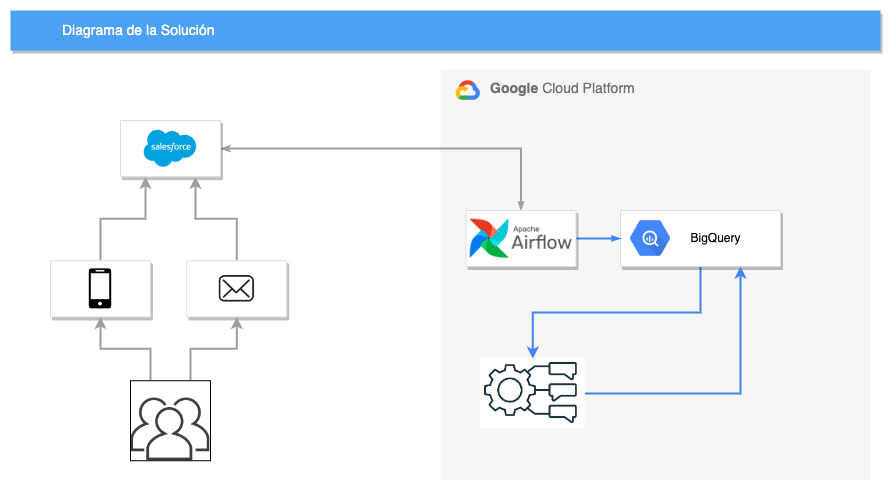
\includegraphics[width=.85\textwidth]{./Figuras/figura1.png}
\caption{Diagrama de alto nivel.}
\label{fig:figura1}
\end{figure}

%\vspace{25px}

Con este proyecto se busca desarrollar y entrenar un modelo clasificador, con los casos de 2021 y 2022 que se encuentran en BigQuery y hayan sido etiquetados manualmente. Una vez desarrollado, se desplegará en la misma nube para realizar las inferencias sobre los nuevos reclamos.

Acerca de la empresa:

Ualá es una \textit{fintech} argentina que brinda su servicio de billetera digital a través de una aplicación móvil. Además, provee una tarjeta prepaga Mastercard para poder operar la cuenta. Los servicios principales que provee son:
\begin{itemize}
	\item Enviar y recibir dinero desde cualquier cuenta bancaria.
	\item Realizar compras nacionales o internacionales con la tarjeta.
	\item Extraer efectivo.
	\item Pagar servicios.
	\item Pedir préstamos o cuotificar consumos.
	\item Realizar ventas a través de \textit{mPOS}, \textit{QR} o link de pago.
	\item Realizar inversiones.
\end{itemize}

%\end{consigna}



\section{2. Identificación y análisis de los interesados}
\label{sec:interesados}




\begin{table}[ht]
%\caption{Identificación de los interesados}
%\label{tab:interesados}
\begin{tabularx}{\linewidth}{@{}|l|X|l|l|@{}}
\hline
\rowcolor[HTML]{C0C0C0} 
Rol           & Nombre y Apellido & Organización 	& Puesto 	\\ \hline
%Auspiciante   &                   &              	&        	\\ \hline
Cliente       & \clientename   & \empclientename	& Gerente de Machine Learning       	\\ \hline
Impulsor      & \clientename   & \empclientename    & Gerente de Machine Learning       	\\ \hline
Responsable   & \authorname       & FIUBA        	& Alumno 	\\ \hline
%Colaboradores &                   &              	&        	\\ \hline
Orientador    & \supname	      & \pertesupname 	& Director Trabajo final \\ \hline
%Equipo        & -                 & -             	& -       	\\ \hline
%Opositores    &                   &              	&        	\\ \hline
Usuario final & Área de atención al cliente        & \empclientename            	& -       	\\ \hline
\end{tabularx}
\end{table}


\begin{itemize}
	\item Impulsor: está interesado en los \textit{insights} que pueda darle este proyecto a nivel tecnológico.
	\item Orientador: cuenta con una gran experiencia en PNL y tiene buena predisposición.
\end{itemize}



\section{3. Propósito del proyecto}
\label{sec:proposito}

%\begin{consigna}{red}
Optimizar el tiempo que lleva el proceso de clasificación de reclamos y consultas mediante su automatización; y por otro lado, reducir la cantidad de personas necesarias para supervisar esta tarea, de manera tal que puedan enfocarse en el proceso de resolución.
%\end{consigna}

\section{4. Alcance del proyecto}
\label{sec:alcance}

%\begin{consigna}{red}
El alcance de este proyecto está orientado a desarrollar un prototipo de solución de software que incluirá las siguientes actividades:

\begin{itemize}
	\item Obtención de los datos: se corresponde con el análisis de las fuentes de datos disponibles y su integración al proceso que se plantea desarrollar.
	\item Análisis exploratorio de los datos: se corresponde con las actividades necesarias para generar nuevos \textit{insights}, que sirvan para guiar el desarrollo de los modelos.
	\item Modelado: se corresponde con la generación de variables a partir de los datos disponibles, que luego serán utilizadas para entrenar los modelos. 
	\item Entrenamiento: se corresponde con la generación de distintos modelos de IA, y su comparación a través de métricas, para encontrar el que mejor se adapte a la problemática de negocio. Estas comparaciones se presentarán en un informe de resultados de los modelos.
	\item Despliegue: se corresponde con el diseño de la infraestructura necesaria para ejecutar los modelos de IA y su despliegue en un entorno de desarrollo (no productivo).
	\item Documentación: se corresponde con los documentos de soporte que explican el proceso de modelado, entrenamiento y despliegue de los modelos.
\end{itemize}

El presente proyecto no incluye:

\begin{itemize}
	\item La adaptación de los modelos a nuevas categorías de reclamos que puedan surgir durante el desarrollo o una vez finalizado el desarrollo. Se utilizarán casos resueltos de 2021 y 2022 y las categorías a considerar serán las que existan hasta ese momento. 
	\item La integración de los modelos y su despliegue con el ambiente productivo.
	\item El soporte de la infraestructura desplegada en el entorno de desarrollo.
\end{itemize}

%\end{consigna}


\section{5. Supuestos del proyecto}
\label{sec:supuestos}

%\begin{consigna}{red}
Para el desarrollo del presente proyecto se supone que:

\begin{itemize}
	\item La empresa mantendrá sus operaciones al menos hasta finalizar el desarrollo.
	\item Se Mantendrá la relación laboral con la empresa al menos hasta finalizar el desarrollo.
	\item El desarrollador asignado a este proyecto no tendrá enfermedades graves que puedan alterar los plazos estipulados para las actividades planteadas.
	\item El área de atención al cliente no realizará cambios en su \textit{CRM} que puedan afectar el proceso de réplica de los casos hacia BigQuery, ni que puedan afectar las categorías sobre las cuales se desarrollan los modelos.
	\item El área de Data de la empresa no cambiará su \textit{Cloud Provider} ni modificará su proceso de réplica hacia BigQuery.
	\item Se tendrá acceso a infraestructura cloud para el entrenamiento y despliegue de los modelos.
	\item Las consultas realizadas al área de atención al cliente se resolverán en plazos razonables.
	
\end{itemize}

%\end{consigna}

\section{6. Requerimientos}
\label{sec:requerimientos}

%\begin{consigna}{red}
\begin{enumerate}
	\item Requerimientos funcionales
		\begin{enumerate}
			\item El sistema debe poder detectar la categoría de un reclamo escrito en lenguaje natural.
			\item El sistema debe poder detectar la categoría de una consulta escrita en lenguaje natural.
			\item El usuario debe poder consumir los resultados de la clasificación desde una base de datos.
			\item El proceso debe ser capaz de interpretar errores de ortografía.
			\item El proceso debe ser capaz de adaptarse a distinta cantidad de palabras en el mensaje.
			\item La solución debe ejecutarse en forma \textit{batch}, corriendo diariamente y tomando los casos del día anterior.
		\end{enumerate}
	\item Requerimientos no funcionales
		\begin{enumerate}
			\item El sistema debe estar desarrollado en lenguaje Python.
			\item El código debe ser versionado con Git.
			\item La solución debe estar desplegada sobre infraestructura de Google Cloud Platform.
			\item La salida de los modelos debe ser almacenada en BigQuery.
			\item El proceso debe ser ejecutado a través del orquestador Apache Airflow.
		\end{enumerate}
	\item Requerimientos de testing
		\begin{enumerate}
			\item Se deben generar métricas de performance de los modelos con el dataset de entrenamiento y de prueba.
		\end{enumerate}
	\item Requerimientos de documentación
		\begin{enumerate}
			\item Se debe confeccionar un documento con el diseño de la arquitectura de alto nivel.
			\item Se debe confeccionar un documento con el diseño de los modelos de IA.
			\item Se debe confeccionar un documento que especifique los datos que consumen los modelos y su origen.
		\end{enumerate}
\end{enumerate}

%\end{consigna}

\section{7. Historias de usuarios (\textit{Product backlog})}
\label{sec:backlog}

%\begin{consigna}{red}
Roles:
\begin{itemize}
	\item Área de atención al cliente
	\item Área de Machine Learning
\end{itemize}

Historias de usuario:

\begin{enumerate}
	\item Como Área de atención al cliente quiero clasificar automáticamente los reclamos y consultas para poder brindar una mejor atención a los usuarios.
	\item Como Área de atención al cliente quiero que el proceso corra diariamente para poder clasificar los reclamos a día cerrado.
	\item Como Área de atención al cliente quiero poder consumir los resultados de la clasificación desde una base de datos para poder integrarlo con el sistema que usamos en el área.
	\item Como Área de Machine Learning quiero tener documentación que detallen la implementación de la solución para que el proyecto se ajuste a nuestras prácticas de desarrollo.
	\item Como Área de Machine Learning quiero tener métricas de performance de los modelos para tener una referencia y poder monitorear desvíos en el proceso en el futuro.
	
\end{enumerate}

Criterio para calcular los \textit{story points} de cada historia:

\begin{itemize}
	\item Criterio A: Cantidad de trabajo a realizar
	\item Criterio B: Complejidad del trabajo a realizar
	\item Criterio C: Incertidumbre del trabajo a realizar
\end{itemize}

Pesos para los criterios:

\begin{table}[H]
\begin{tabular}{c c c c}
\hline
\rowcolor[HTML]{C0C0C0} 
Nivel           & Criterio A     & Criterio B 	    & Criterio C 	 \\ \hline
Bajo            & 1              & 1	            & 1              \\ \hline
Medio           & 2              & 3                & 5               \\ \hline
Alto            & 5              & 5        	    & 8 	          \\ \hline
\end{tabular}
\end{table}

Story points:

\begin{table}[H]
\begin{tabular}{c c c c c c}
\hline
\rowcolor[HTML]{C0C0C0} 
Historia           & Criterio A     & Criterio B 	    & Criterio C   & Peso resultante  & Fibonacci	 \\ \hline
1                  & 5              & 5	                & 8            &  18              &  21            \\ \hline
2                  & 2              & 1                 & 1            &  4               &  5            \\ \hline
3                  & 2              & 3        	        & 1 	       &  6               &  8              \\ \hline
4                  & 2              & 1        	        & 1 	       &  4               &  5             \\ \hline
5                  & 2              & 3        	        & 1 	       &  6               &  8              \\ \hline
\end{tabular}
\end{table}

%\end{consigna}

\section{8. Entregables principales del proyecto}
\label{sec:entregables}

%\begin{consigna}{red}

Los entregables del proyecto son:

\begin{itemize}
	\item Plan de proyecto.
	\item Código fuente (queda reservado para \empclientename).
	\item Modelos de inteligencia artificial (queda reservado para \empclientename).
	\item Documento con el diseño de arquitectura de alto nivel.
	\item Documento con el diseño de los modelos de inteligencia artificial.
	\item Documento que especifica los datos que consumen los modelos y su origen.
	\item Documento con las métricas de evaluación de los modelos.
	\item Informe de avance.
	\item Memoria del trabajo.
\end{itemize}

%\end{consigna}

\section{9. Desglose del trabajo en tareas}
\label{sec:wbs}

%\begin{consigna}{red}
Se detallan a continuación todas las actividades que se harán en el proyecto para dar cumplimiento a los requerimientos y su duración estimada:

\begin{enumerate}
	\item Planificación general del proyecto (50 h)
		\begin{enumerate}
			\item Redacción de la descripción técnica-conceptual y propósito. (10 h)
			\item Definición del alcance, requerimientos y entregables. (10 h)
			\item Definición de tiempos y presupuesto. (15 h)
			\item Definición de la gestión de riesgos, calidad y procesos de cierre. (15 h)
		\end{enumerate}
	\item Relevamiento (30 h)
		\begin{enumerate}
			\item Reuniones con el área de atención al cliente. (10 h)
			\item Análisis de las fuentes de datos. (10 h)
			\item Análisis del proceso de clasificación de reclamos y consultas. (10 h)
		\end{enumerate}
	\item Análisis exploratorio de los datos (35 h)
		\begin{enumerate}
			\item Análisis de la distribución de categorías. (10 h) 
			\item Análisis de la longitud de los mensajes. (10 h)
			\item Análisis del procesamiento del texto. (15 h)
		\end{enumerate}
	\item Desarrollo (290 h)
		\begin{enumerate}
			\item Programación de \textit{scripts} para obtener datos de entrada de los modelos. (10 h)
			\item Desarrollo del pipeline de preprocesamiento del texto. (90 h)
				\begin{itemize}
					\item Módulo para remover partes comunes de los mensajes. (15 h)
					\item Módulo para remover palabras redundantes. (15 h)
					\item Módulo para remover símbolos. (10 h)
					\item Módulo para corregir faltas de ortografía. (40 h)
					\item Módulo para armar secuencias. (10 h)
				\end{itemize}
			\item Desarrollo y entrenamiento de \textit{embeddings}. (60 h)
				\begin{itemize}
					\item Investigación herramientas de embeddings. (20 h)
					\item Selección de herramienta de embeddings. (20 h)
					\item Entrenamiento de embeddings. (20 h)
				\end{itemize}
			\item Desarrollo y entrenamiento de modelos. (130 h)
				\begin{itemize}
					\item Investigación de arquitecturas de IA que apliquen al problema. (40 h)
					\item Entrenamiento de modelo baseline. (10 h)
					\item Desarrollo de \textit{scripts} para modelos avanzados. (25 h)
					\item Entrenamiento de modelos avanzados. (50 h)
					\item Desarrollo de módulo de escritura de resultados en BigQuery. (5 h)
				\end{itemize}
		\end{enumerate}
	\item Evaluación y pruebas (35 h)
		\begin{enumerate}
			\item Obtención de métricas de los modelos. (30 h)
			\item Selección del mejor modelo. (5 h)
		\end{enumerate}
	\item Despliegue (50 h)
		\begin{enumerate}
			\item Diseño de la arquitectura del \textit{pipeline}. (10 h)
			\item Desarrollo de Github Actions. (5 h)
			\item Desarrollo de la imagen de Docker. (20 h)
			\item Desarrollo de DAG de clasificación. (15 h)
		\end{enumerate}
	\item Documentación (30 h)
		\begin{enumerate}
			\item Elaboración de documento de arquitectura alto nivel. (10 h)
			\item Elaboración de documento con el diseño de los modelos de IA. (10 h)
			\item Elaboración de documento con los datos consumidos. (10 h)
		\end{enumerate}
	\item Cierre del proyecto (80 h)
		\begin{enumerate}
			\item Redacción del informe de avance. (20 h)
			\item Redacción de memoria final. (40 h)
			\item Elaboración de presentación para exposición final. (20 h) 
		\end{enumerate}
\end{enumerate}

Cantidad total de horas: (600 h)

%\end{consigna}

\section{10. Diagrama de Activity On Node}
\label{sec:AoN}

\begin{consigna}{red}
Armar el AoN a partir del WBS definido en la etapa anterior. 

%La figura \ref{fig:AoN} fue elaborada con el paquete latex tikz y pueden consultar la siguiente referencia \textit{online}:

%\url{https://www.overleaf.com/learn/latex/LaTeX_Graphics_using_TikZ:_A_Tutorial_for_Beginners_(Part_3)\%E2\%80\%94Creating_Flowcharts}

\end{consigna}

\begin{figure}[htpb]
\centering 
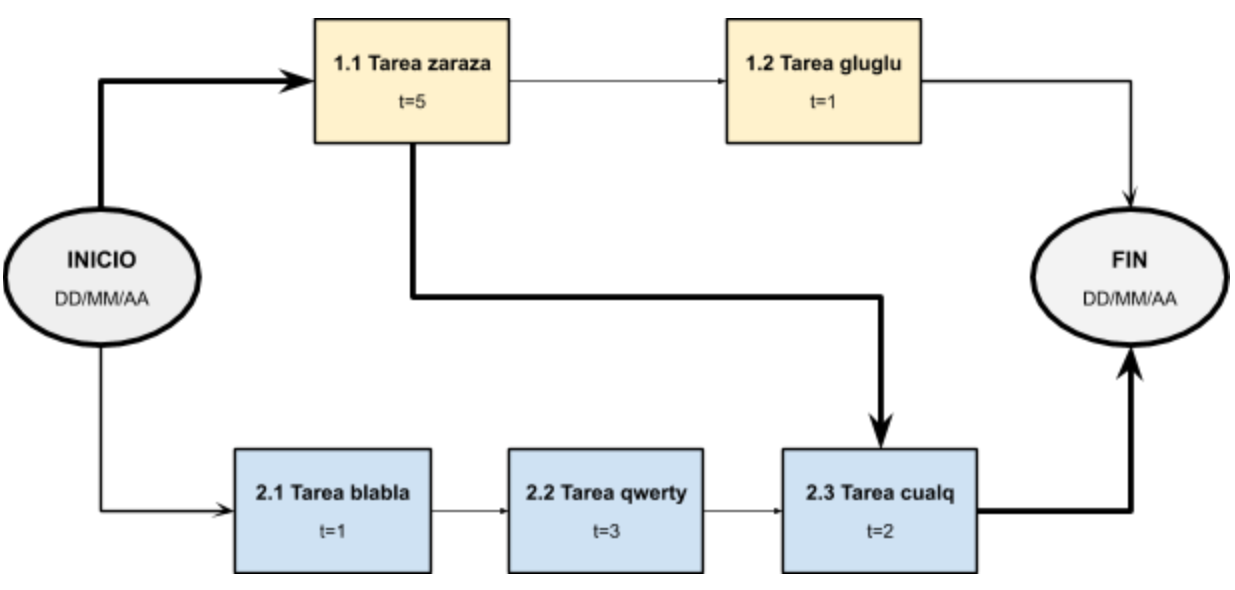
\includegraphics[width=.8\textwidth]{./Figuras/AoN.png}
\caption{Diagrama de \textit{Activity on Node}.}
\label{fig:AoN}
\end{figure}

Indicar claramente en qué unidades están expresados los tiempos.
De ser necesario indicar los caminos semicríticos y analizar sus tiempos mediante un cuadro.
Es recomendable usar colores y un cuadro indicativo describiendo qué representa cada color, como se muestra en el siguiente ejemplo:



\section{11. Diagrama de Gantt}
\label{sec:gantt}

\begin{consigna}{red}

Existen muchos programas y recursos \textit{online} para hacer diagramas de Gantt, entre los cuales destacamos:

\begin{itemize}
\item Planner
\item GanttProject
\item Trello + \textit{plugins}. En el siguiente link hay un tutorial oficial: \\ \url{https://blog.trello.com/es/diagrama-de-gantt-de-un-proyecto}
\item Creately, herramienta online colaborativa. \\\url{https://creately.com/diagram/example/ieb3p3ml/LaTeX}
\item Se puede hacer en latex con el paquete \textit{pgfgantt}\\ \url{http://ctan.dcc.uchile.cl/graphics/pgf/contrib/pgfgantt/pgfgantt.pdf}
\end{itemize}

Pegar acá una captura de pantalla del diagrama de Gantt, cuidando que la letra sea suficientemente grande como para ser legible. 
Si el diagrama queda demasiado ancho, se puede pegar primero la ``tabla'' del Gantt y luego pegar la parte del diagrama de barras del diagrama de Gantt.

Configurar el software para que en la parte de la tabla muestre los códigos del EDT (WBS).\\
Configurar el software para que al lado de cada barra muestre el nombre de cada tarea.\\
Revisar que la fecha de finalización coincida con lo indicado en el Acta Constitutiva.

En la figura \ref{fig:gantt}, se muestra un ejemplo de diagrama de Gantt realizado con el paquete de \textit{pgfgantt}. En la plantilla pueden ver el código que lo genera y usarlo de base para construir el propio.

\begin{figure}[htbp]
\begin{center}
\begin{ganttchart}{1}{12}
  \gantttitle{2020}{12} \\
  \gantttitlelist{1,...,12}{1} \\
  \ganttgroup{Group 1}{1}{7} \\
  \ganttbar{Task 1}{1}{2} \\
  \ganttlinkedbar{Task 2}{3}{7} \ganttnewline
  \ganttmilestone{Milestone o hito}{7} \ganttnewline
  \ganttbar{Final Task}{8}{12}
  \ganttlink{elem2}{elem3}
  \ganttlink{elem3}{elem4}
\end{ganttchart}
\end{center}
\caption{Diagrama de Gantt de ejemplo}
\label{fig:gantt}
\end{figure}


\begin{landscape}
\begin{figure}[htpb]
\centering 
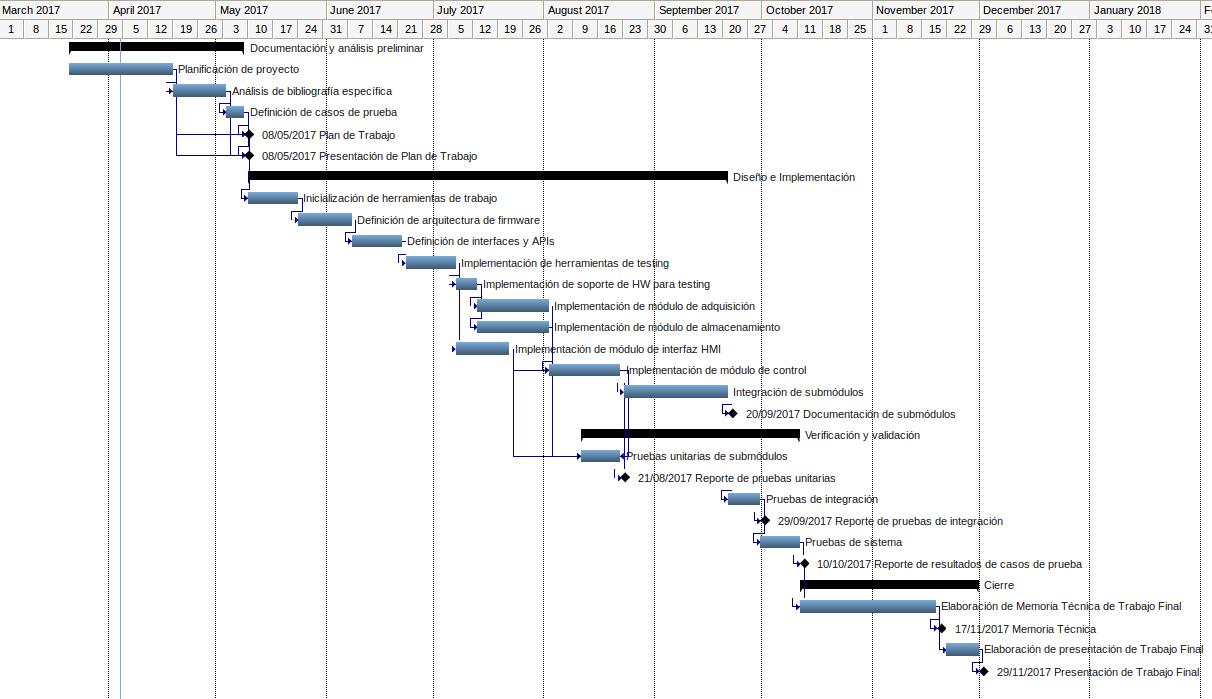
\includegraphics[height=.85\textheight]{./Figuras/Gantt-2.png}
\caption{Ejemplo de diagrama de Gantt rotado}
\label{fig:diagGantt}
\end{figure}

\end{landscape}

\end{consigna}


\section{12. Presupuesto detallado del proyecto}
\label{sec:presupuesto}

\begin{consigna}{red}
Si el proyecto es complejo entonces separarlo en partes:
\begin{itemize}
	\item Un total global, indicando el subtotal acumulado por cada una de las áreas.
	\item El desglose detallado del subtotal de cada una de las áreas.
\end{itemize}

IMPORTANTE: No olvidarse de considerar los COSTOS INDIRECTOS.

\end{consigna}

\begin{table}[htpb]
\centering
\begin{tabularx}{\linewidth}{@{}|X|c|r|r|@{}}
\hline
\rowcolor[HTML]{C0C0C0} 
\multicolumn{4}{|c|}{\cellcolor[HTML]{C0C0C0}COSTOS DIRECTOS} \\ \hline
\rowcolor[HTML]{C0C0C0} 
Descripción &
  \multicolumn{1}{c|}{\cellcolor[HTML]{C0C0C0}Cantidad} &
  \multicolumn{1}{c|}{\cellcolor[HTML]{C0C0C0}Valor unitario} &
  \multicolumn{1}{c|}{\cellcolor[HTML]{C0C0C0}Valor total} \\ \hline
 &
  \multicolumn{1}{c|}{} &
  \multicolumn{1}{c|}{} &
  \multicolumn{1}{c|}{} \\ \hline
 &
  \multicolumn{1}{c|}{} &
  \multicolumn{1}{c|}{} &
  \multicolumn{1}{c|}{} \\ \hline
\multicolumn{1}{|l|}{} &
   &
   &
   \\ \hline
\multicolumn{1}{|l|}{} &
   &
   &
   \\ \hline
\multicolumn{3}{|c|}{SUBTOTAL} &
  \multicolumn{1}{c|}{} \\ \hline
\rowcolor[HTML]{C0C0C0} 
\multicolumn{4}{|c|}{\cellcolor[HTML]{C0C0C0}COSTOS INDIRECTOS} \\ \hline
\rowcolor[HTML]{C0C0C0} 
Descripción &
  \multicolumn{1}{c|}{\cellcolor[HTML]{C0C0C0}Cantidad} &
  \multicolumn{1}{c|}{\cellcolor[HTML]{C0C0C0}Valor unitario} &
  \multicolumn{1}{c|}{\cellcolor[HTML]{C0C0C0}Valor total} \\ \hline
\multicolumn{1}{|l|}{} &
   &
   &
   \\ \hline
\multicolumn{1}{|l|}{} &
   &
   &
   \\ \hline
\multicolumn{1}{|l|}{} &
   &
   &
   \\ \hline
\multicolumn{3}{|c|}{SUBTOTAL} &
  \multicolumn{1}{c|}{} \\ \hline
\rowcolor[HTML]{C0C0C0}
\multicolumn{3}{|c|}{TOTAL} &
   \\ \hline
\end{tabularx}%
\end{table}


\section{13. Gestión de riesgos}
\label{sec:riesgos}

\begin{consigna}{red}
a) Identificación de los riesgos (al menos cinco) y estimación de sus consecuencias:
 
Riesgo 1: detallar el riesgo (riesgo es algo que si ocurre altera los planes previstos de forma negativa)
\begin{itemize}
	\item Severidad (S): mientras más severo, más alto es el número (usar números del 1 al 10).\\
	Justificar el motivo por el cual se asigna determinado número de severidad (S).
	\item Probabilidad de ocurrencia (O): mientras más probable, más alto es el número (usar del 1 al 10).\\
	Justificar el motivo por el cual se asigna determinado número de (O). 
\end{itemize}   

Riesgo 2:
\begin{itemize}
	\item Severidad (S): 
	\item Ocurrencia (O):
\end{itemize}

Riesgo 3:
\begin{itemize}
	\item Severidad (S): 
	\item Ocurrencia (O):
\end{itemize}


b) Tabla de gestión de riesgos:      (El RPN se calcula como RPN=SxO)

\begin{table}[htpb]
\centering
\begin{tabularx}{\linewidth}{@{}|X|c|c|c|c|c|c|@{}}
\hline
\rowcolor[HTML]{C0C0C0} 
Riesgo & S & O & RPN & S* & O* & RPN* \\ \hline
       &   &   &     &    &    &      \\ \hline
       &   &   &     &    &    &      \\ \hline
       &   &   &     &    &    &      \\ \hline
       &   &   &     &    &    &      \\ \hline
       &   &   &     &    &    &      \\ \hline
\end{tabularx}%
\end{table}

Criterio adoptado: 
Se tomarán medidas de mitigación en los riesgos cuyos números de RPN sean mayores a...

Nota: los valores marcados con (*) en la tabla corresponden luego de haber aplicado la mitigación.

c) Plan de mitigación de los riesgos que originalmente excedían el RPN máximo establecido:
 
Riesgo 1: plan de mitigación (si por el RPN fuera necesario elaborar un plan de mitigación).
  Nueva asignación de S y O, con su respectiva justificación:
  - Severidad (S): mientras más severo, más alto es el número (usar números del 1 al 10).
          Justificar el motivo por el cual se asigna determinado número de severidad (S).
  - Probabilidad de ocurrencia (O): mientras más probable, más alto es el número (usar del 1 al 10).
          Justificar el motivo por el cual se asigna determinado número de (O).

Riesgo 2: plan de mitigación (si por el RPN fuera necesario elaborar un plan de mitigación).
 
Riesgo 3: plan de mitigación (si por el RPN fuera necesario elaborar un plan de mitigación).

\end{consigna}


\section{14. Gestión de la calidad}
\label{sec:calidad}

\begin{consigna}{red}
Para cada uno de los requerimientos del proyecto indique:
\begin{itemize} 
\item Req \#1: copiar acá el requerimiento.

\begin{itemize}
	\item Verificación para confirmar si se cumplió con lo requerido antes de mostrar el sistema al cliente. Detallar 
	\item Validación con el cliente para confirmar que está de acuerdo en que se cumplió con lo requerido. Detallar  
\end{itemize}

\end{itemize}

Tener en cuenta que en este contexto se pueden mencionar simulaciones, cálculos, revisión de hojas de datos, consulta con expertos, mediciones, etc.  Las acciones de verificación suelen considerar al entregable como ``caja blanca'', es decir se conoce en profundidad su funcionamiento interno.  En cambio, las acciones de validación suelen considerar al entregable como ``caja negra'', es decir, que no se conocen los detalles de su funcionamiento interno.

\end{consigna}

\section{15. Procesos de cierre}    
\label{sec:cierre}

\begin{consigna}{red}
Establecer las pautas de trabajo para realizar una reunión final de evaluación del proyecto, tal que contemple las siguientes actividades:

\begin{itemize}
	\item Pautas de trabajo que se seguirán para analizar si se respetó el Plan de Proyecto original:
	 - Indicar quién se ocupará de hacer esto y cuál será el procedimiento a aplicar. 
	\item Identificación de las técnicas y procedimientos útiles e inútiles que se emplearon, y los problemas que surgieron y cómo se solucionaron:
	 - Indicar quién se ocupará de hacer esto y cuál será el procedimiento para dejar registro.
	\item Indicar quién organizará el acto de agradecimiento a todos los interesados, y en especial al equipo de trabajo y colaboradores:
	  - Indicar esto y quién financiará los gastos correspondientes.
\end{itemize}

\end{consigna}


\end{document}
